\documentclass[11pt]{article}

% ---------- Packages ----------
\usepackage[a4paper,margin=1in]{geometry}
\usepackage{amsmath,amssymb,amsthm,mathtools}
\usepackage{physics} % \dd, \partial, etc.
\usepackage{microtype}
\usepackage{enumitem}
\setlist{nosep}
\usepackage{tikz}
\usetikzlibrary{arrows.meta,calc,angles,quotes,decorations.pathreplacing,patterns}
\usepackage{pgfplots}
\pgfplotsset{compat=1.18}

% ---------- Macros ----------
\newcommand{\C}{\mathbb{C}}
\newcommand{\Z}{\mathbb{Z}}
\newcommand{\R}{\mathbb{R}}
\newcommand{\ii}{\mathrm{i}}
\newcommand{\dz}{\,\mathrm{d}z}
\newcommand{\dx}{\,\mathrm{d}x}
\newcommand{\dy}{\,\mathrm{d}y}
\newcommand{\dbarz}{\,\mathrm{d}\bar z}
\newcommand{\T}{\mathbb{T}}
\newcommand{\pp}{\wp}
\newcommand{\ppp}{\wp'}
\newcommand{\e}{\mathrm{e}}
%\DeclareMathOperator{\Res}{Res}
\DeclareMathOperator{\Impart}{Im}
\DeclareMathOperator{\Repart}{Re}

\newtheorem{definition}{Definition}
\newtheorem{remark}{Remark}
\newtheorem{proposition}{Proposition}
\newtheorem{example}{Example}
\newtheorem{exercise}{Exercise}

% ---------- Title ----------
\title{\Large Part II — Building the Weierstrass $\wp$-Function from the Holomorphic Form $dt=\omega$}
\author{ }
\date{ }

\begin{document}
	\maketitle
	
	\section*{Roadmap}
	Starting with the flat holomorphic $1$-form \(dz\) on \(\C\), we pass to the complex torus \(X=\C/\Lambda\) and its nowhere-vanishing $1$-form \(\omega\) induced by \(dz\). Fix cycles \(a,b\) so that \(\int_a\omega=1,\ \int_b\omega=\tau\) with \(\Impart\,\tau>0\). Using the Abel coordinate \(t\) defined by \(dt=\omega\), we \emph{define} the Weierstrass function by a lattice sum in $t$, derive its differential equation via Eisenstein series, and identify the elliptic curve \(y^2=4x^3-g_2x-g_3\). TikZ figures illustrate periods, poles, and the cubic.
	
	\section{From the torus and its $1$-form to the Abel coordinate}
	Let \(\Lambda=\Z+\tau\Z\subset\C\) with \(\Impart\,\tau>0\). The quotient \(X=\C/\Lambda\) is a complex torus. The standard $1$-form \(dz\) is $\Lambda$-invariant, hence descends to a holomorphic $1$-form \(\omega\) on \(X\) that has \emph{no zeros}. Choose homology generators \(a,b\) represented by the edges of a fundamental parallelogram. Normalize so that
	\[
	\int_a\omega=1,\qquad \int_b\omega=\tau.
	\]
	\begin{definition}[Abel coordinate]
		On the universal cover \(\C\to X\), choose a lift near \(0\) and define \(t\) by \(dt=\omega\). Thus on the cover one may take \(t=z+\mathrm{const}\), so that $a$- and $b$-periods are \(1,\tau\).
	\end{definition}
	
	\begin{center}
		\begin{tikzpicture}[scale=1.05]
			% vertices of fundamental parallelogram
			\coordinate (O) at (0,0);
			\coordinate (A) at (3,0);
			\coordinate (T) at (1.2,2.0); % vector tau ~ (Re, Im)
			\coordinate (B) at ($(A)+(T)$);
			% parallelogram and lattice
			\draw[very thick] (O) -- (A) -- (B) -- (T) -- cycle;
			\foreach \m in {-2,...,3} {
				\foreach \n in {-2,...,2} {
					\fill ($(O) + \m*(A) + \n*(T)$) circle (1pt);
				}
			}
			% edges arrows
			\draw[very thick,-{Latex[length=3mm]}] (O) -- (A) node[midway,below] {$a$};
			\draw[very thick,-{Latex[length=3mm]}] (O) -- (T) node[midway,left] {$b$};
			% labels
			\node at ($(A)!0.5!(B)+(0,-0.5)$) {$\int_a \omega = 1$};
			\node at ($(T)!0.5!(B)+(-0.6,0.0)$) {$\int_b \omega = \tau$};
			\node at (4.8,2.5) {\small Fundamental parallelogram for $\Lambda=\Z+\tau\Z$};
		\end{tikzpicture}
		
		\smallskip
		\small Fig.~1. Periods of \(\omega\) along $a,b$ in the Abel coordinate \(t\).
	\end{center}
	
	\section{Defining $\wp$ from \(dt=\omega\)}
	\begin{definition}[Weierstrass function and its derivative]
		With \(t\) as above and \(\Lambda\) fixed, define
		\[
		\boxed{\quad
			\pp(t;\Lambda)=\frac{1}{t^2}+\sum_{\lambda\in\Lambda\setminus\{0\}}
			\left(\frac{1}{(t-\lambda)^2}-\frac{1}{\lambda^2}\right),\qquad
			\ppp(t)=-\frac{2}{t^3}-2\sum_{\lambda\neq 0}\frac{1}{(t-\lambda)^3}.
			\quad}
		\]
	\end{definition}
	
	\begin{proposition}[Basic properties]
		\(\pp\) is doubly periodic with respect to \(\Lambda\), even, and has a double pole at each \(\lambda\in\Lambda\) with no residues. Its derivative \(\ppp\) is odd and vanishes exactly at the three (nonzero) half-periods modulo sign.
	\end{proposition}
	\begin{proof}[Sketch]
		Absolute convergence of the modified sum follows by pairing \(\lambda\) and $-\lambda$. Periodicity follows from invariance under \(t\mapsto t+\lambda\). Even/odd are immediate from the definitions. Residues vanish by symmetry, hence $\pp$ is elliptic (doubly periodic meromorphic).
	\end{proof}
	
	\begin{center}
		\begin{tikzpicture}[scale=1.02]
			% lattice
			\coordinate (O) at (0,0);
			\coordinate (A) at (3,0);
			\coordinate (T) at (1.2,2.0);
			\foreach \m in {-2,...,2} {
				\foreach \n in {-2,...,2} {
					\fill ($(O) + \m*(A) + \n*(T)$) circle (1pt);
				}
			}
			% mark poles
			\foreach \m in {-1,0,1} {
				\foreach \n in {-1,0,1} {
					\draw[thick] ($(O)+\m*(A)+\n*(T)$) circle (0.18);
				}
			}
			\node at (4.8,2.5) {\small Poles of $\pp$ at the lattice points (double, residue $0$).};
		\end{tikzpicture}
		
		\smallskip
		\small Fig.~2. The pole lattice of \(\pp\).
	\end{center}
	
	\section{Eisenstein series and the cubic differential equation}
	Define Eisenstein series (absolutely convergent for \(k\ge 2\)):
	\[
	G_{2k}(\Lambda)=\sum_{\lambda\in\Lambda\setminus\{0\}}\frac{1}{\lambda^{2k}},\qquad
	g_2=60\,G_4,\quad g_3=140\,G_6.
	\]
	Then the Laurent expansion around \(t=0\) is
	\[
	\pp(t)=\frac{1}{t^2}+3G_4\,t^2+5G_6\,t^4+7G_8\,t^6+\cdots.
	\]
	\begin{proposition}[Weierstrass equation]
		\[
		\boxed{\qquad (\pp'(t))^2\;=\;4\,\pp(t)^3 - g_2\,\pp(t) - g_3.\qquad}
		\]
	\end{proposition}
	\begin{proof}[Sketch]
		The function \(F(t)=(\pp')^2-4\pp^3+g_2\pp+g_3\) is elliptic with no poles by checking its Laurent series at \(t=0\). By Liouville for elliptic functions, \(F\) is constant, and matching the constant term in the expansion forces the constant to be \(0\).
	\end{proof}
	
	\section{Uniformization and the elliptic curve}
	Let \(x=\pp(t)\), \(y=\pp'(t)\). Then \((x(t),y(t))\) lies on the cubic
	\[
	E: \quad y^2=4x^3-g_2x-g_3.
	\]
	\begin{proposition}[Differentials match]
		Under \(t\mapsto (x(t),y(t))\), the holomorphic differential \(\omega=dt\) corresponds to
		\[
		dt=\frac{dx}{y}\quad\text{on }E.
		\]
	\end{proposition}
	\begin{proof}
		Differentiate \(x=\pp(t)\) to get \(dx=\pp'(t)\,dt=y\,dt\).
	\end{proof}
	\begin{remark}[Inverse via an elliptic integral]
		Conversely,
		\[
		t=\int^x \frac{dx}{\sqrt{\,4x^3-g_2x-g_3\,}},
		\]
		recovering the Abel coordinate from the cubic.
	\end{remark}
	
	\begin{center}
		\begin{tikzpicture}[scale=1.0]
			% A qualitative elliptic curve y^2 = 4x^3 - g2 x - g3 (scaled example)
			\begin{axis}[
				width=11cm,height=5.5cm,
				axis lines=middle,
				xlabel={$x$}, ylabel={$y$},
				xmin=-3.2,xmax=3.2,ymin=-4.5,ymax=4.5,
				samples=400, domain=-3:3, smooth, no markers,
				xtick=\empty, ytick=\empty
				]
				% choose a simple scaled model with g2=1, g3=0 to illustrate
				\addplot+[very thick] ({x},{ sqrt(max(0,4*x^3 - x)) });
				\addplot+[very thick] ({x},{-sqrt(max(0,4*x^3 - x)) });
			\end{axis}
			\node at (10.4,1.3) {\small A representative shape of $y^2=4x^3-g_2x-g_3$};
		\end{tikzpicture}
		
		\smallskip
		\small Fig.~3. The elliptic curve; the map \(t\mapsto (\pp(t),\pp'(t))\) wraps the torus over it.
	\end{center}
	
	\section{Half-period values $e_1,e_2,e_3$}
	Let \(e_1,e_2,e_3\) be the distinct zeros of \(4x^3-g_2x-g_3\) (so \(e_1+e_2+e_3=0\)). They are exactly the values of \(\pp\) at the three nontrivial half-periods \(t=\tfrac12,\ \tfrac{\tau}{2},\ \tfrac{1+\tau}{2}\) (order varies with basis). Equivalently,
	\[
	\pp'(t)=0 \iff t\equiv \tfrac{1}{2},\ \tfrac{\tau}{2},\ \tfrac{1+\tau}{2}\ (\mathrm{mod}\ \Lambda),\qquad
	\pp\bigl(\tfrac{\ast}{2}\bigr)\in\{e_1,e_2,e_3\}.
	\]
	
	\begin{center}
		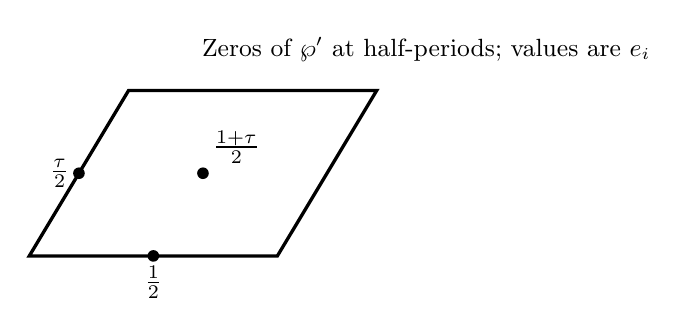
\begin{tikzpicture}[scale=1.05]
			% fundamental parallelogram
			\coordinate (O) at (0,0);
			\coordinate (A) at (3,0);
			\coordinate (T) at (1.2,2.0);
			\coordinate (B) at ($(A)+(T)$);
			\draw[very thick] (O) -- (A) -- (B) -- (T) -- cycle;
			% half period points
			\fill (1.5,0) circle (2pt) node[below] {$\frac12$};
			\fill (0.6,1.0) circle (2pt) node[left] {$\frac{\tau}{2}$};
			\fill (2.1,1.0) circle (2pt) node[above right] {$\frac{1+\tau}{2}$};
			\node at (4.8,2.5) {\small Zeros of $\pp'$ at half-periods; values are $e_i$};
		\end{tikzpicture}
		
		\smallskip
		\small Fig.~4. Half-periods in the fundamental domain; \(\pp'\) vanishes there.
	\end{center}
	
	\section{Two concrete symmetry cases}
	\subsection*{(A) Lemniscatic (square) lattice \(\tau=\ii\)}
	By quarter-turn symmetry \(z\mapsto \ii z\), one shows \(G_6=0\), hence \(g_3=0\). The cubic is
	\[
	y^2=4x^3-g_2 x,\qquad \text{roots } \{e_1,0,-e_1\}.
	\]
	One of the half-period values is \(0\) (indeed \(\pp(\tfrac12+\tfrac{\ii}{2})=0\) up to basis choice). The curve has symmetric ``lemniscatic'' shape.
	
	\subsection*{(B) Equianharmonic (hexagonal) lattice \(\tau=\e^{\ii\pi/3}\)}
	By $60^\circ$ rotational symmetry, \(G_4=0\), hence \(g_2=0\). The cubic is
	\[
	y^2=4x^3-g_3,\qquad \text{roots } \omega\sqrt[3]{\tfrac{g_3}{4}},\ \omega^2\sqrt[3]{\tfrac{g_3}{4}},\ \sqrt[3]{\tfrac{g_3}{4}},\quad (\omega^3=1,\ \omega\neq 1),
	\]
	so the three $e_i$ are the three vertices of a rotated equilateral triple on the $x$-line (in the appropriate real model).
	
	\section{Local expansions and quick computations}
	From the Laurent series,
	\[
	\pp(t)=\frac{1}{t^2}+3G_4 t^2+5G_6 t^4+\cdots,\qquad
	\pp'(t)=-\frac{2}{t^3}-6G_4 t - 20 G_6 t^3 - \cdots.
	\]
	\begin{example}[Sanity check near $t=0$]
		Take a small \(t\) and keep the first two nontrivial terms: \(\pp(t)\approx t^{-2}+3G_4 t^2\), \(\pp'(t)\approx -2t^{-3}-6G_4 t\). Plug into \(y^2=4x^3-g_2x-g_3\); using \(g_2=60G_4\), \(g_3=140G_6\), the first non-canceling terms match identically.
	\end{example}
	
	\section{Why $\omega$ determines everything (and vice versa)}
	- Input: \((X,\omega)\) with \(\int_a\omega=1,\ \int_b\omega=\tau\).  
	- Output: \(\Lambda=\Z+\tau\Z\), Abel coordinate \(t\) with \(dt=\omega\), then \(\pp,\pp'\), then \(g_2,g_3\), then the cubic \(E\).
	- Conversely, given \(E:y^2=4x^3-g_2x-g_3\), the invariant differential \(\dfrac{dx}{y}\) has periods \(1,\tau\), recovering \(\omega\) and \(\Lambda\) (up to scaling).
	
	\section*{Worked ``recipe''}
	\vspace{-0.5em}
	\begin{enumerate}
		\item Pick \(\tau\) with \(\Impart\,\tau>0\), set \(\Lambda=\Z+\tau\Z\).
		\item Define \(t\) by \(dt=\omega\) and periods \(1,\tau\).
		\item Build \(\pp,\pp'\) by lattice sums; compute \(G_4,G_6\), \(g_2,g_3\).
		\item Verify \((\pp')^2=4\pp^3-g_2\pp-g_3\) and locate half-period zeros of \(\pp'\).
		\item Map \(t\mapsto (\pp(t),\pp'(t))\) onto \(E:\ y^2=4x^3-g_2x-g_3\); inverse is \(\displaystyle t=\int\frac{dx}{y}\).
	\end{enumerate}
	
	\section*{Exercises (with short nudges)}
	\begin{enumerate}[label=\arabic*)]
		\item Prove absolute convergence of the modified series for \(\pp\) by pairing \(\lambda\) and \(-\lambda\).
		\item Show that if \(f\) is entire and \(\Lambda\)-periodic then \(f\) is constant (Liouville on a fundamental domain).
		\item For \(\tau=\ii\), prove \(G_6=0\) by symmetry: the six directions of shortest nonzero lattice vectors cancel in the \(6\)-th power sum.
		\item For \(\tau=\e^{\ii\pi/3}\), prove \(G_4=0\) similarly.
		\item Check that \(dt\) equals \(\dfrac{dx}{y}\) by differentiating \(x=\pp(t)\).
	\end{enumerate}
	
\end{document}
